\documentclass[tikz,border=8pt]{standalone}
\usepackage[T1]{fontenc}
\usepackage[utf8]{inputenc}
\usepackage{tikz}
\usetikzlibrary{arrows.meta,positioning,fit}

\begin{document}
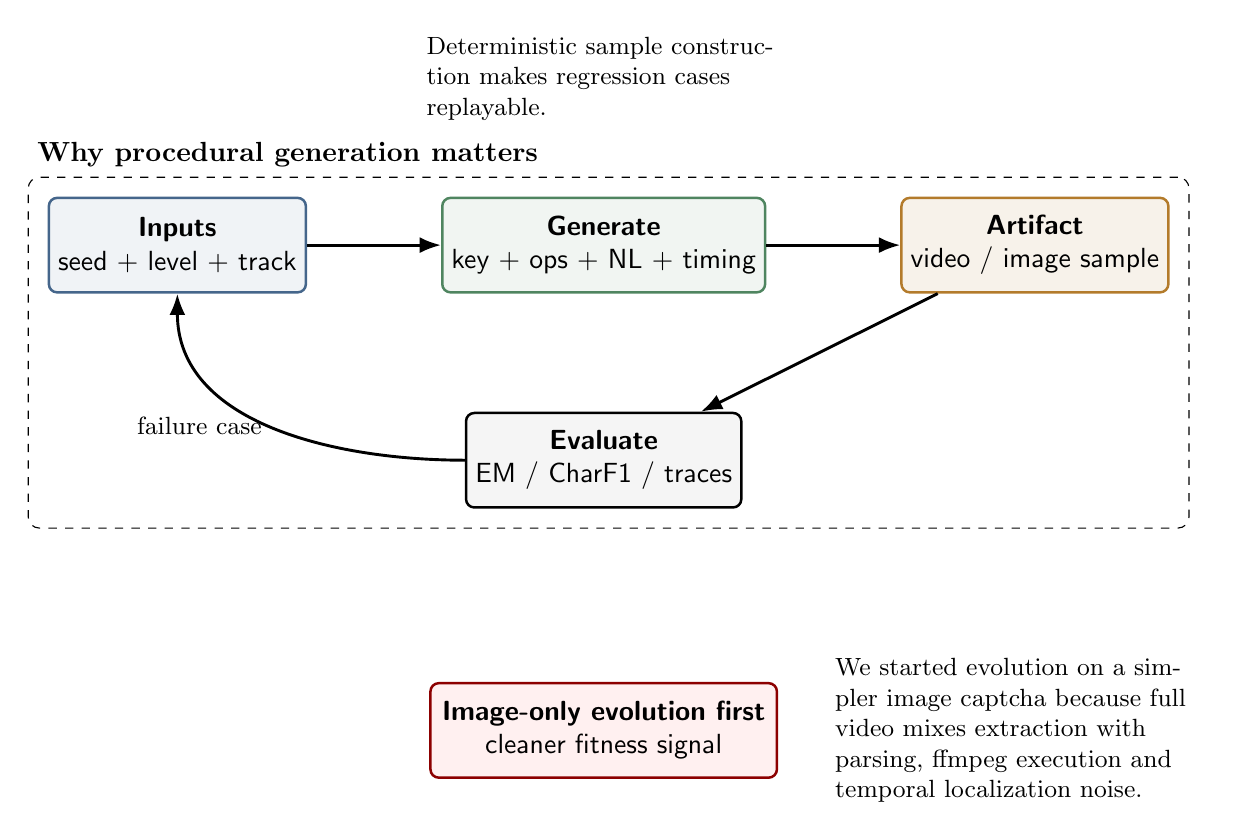
\begin{tikzpicture}[
  font=\sffamily,
  >=Latex,
  box/.style={draw, rounded corners=3pt, minimum width=2.8cm, minimum height=1.2cm, align=center, line width=0.9pt},
  note/.style={font=\small, text width=4.2cm, align=left}
]

\definecolor{c1}{RGB}{69,102,139}
\definecolor{c2}{RGB}{79,133,96}
\definecolor{c3}{RGB}{179,123,43}

\node[box, draw=c1, fill=c1!8] (seed) at (0,0) {\textbf{Inputs}\\seed + level + track};
\node[box, draw=c2, fill=c2!8, right=1.7cm of seed] (sample) {\textbf{Generate}\\key + ops + NL + timing};
\node[box, draw=c3, fill=c3!10, right=1.7cm of sample] (art) {\textbf{Artifact}\\video / image sample};
\node[box, fill=gray!8, below=1.5cm of sample] (eval) {\textbf{Evaluate}\\EM / CharF1 / traces};

\draw[->, line width=1.05pt] (seed) -- (sample);
\draw[->, line width=1.05pt] (sample) -- (art);
\draw[->, line width=1.05pt] (art) -- (eval);
\draw[->, line width=1.05pt] (eval.west) to[out=180,in=-90] node[left, font=\small] {failure case} (seed.south);

\node[note, above=0.85cm of sample, text width=4.5cm] {
Deterministic sample construction makes regression cases replayable.
};

\node[draw, dashed, rounded corners=4pt, inner sep=7pt, fit=(seed)(sample)(art)(eval)] (fitbox) {};
\node[anchor=south west, font=\bfseries] at (fitbox.north west) {Why procedural generation matters};

\node[box, below=2.2cm of eval, minimum width=4.4cm, fill=red!6, draw=red!55!black] (imgmode) {\textbf{Image-only evolution first}\\cleaner fitness signal};
\node[note, right=0.6cm of imgmode, text width=4.6cm] {
We started evolution on a simpler image captcha because full video mixes extraction with parsing, ffmpeg execution and temporal localization noise.
};

\end{tikzpicture}
\end{document}
